\documentclass{report}

\usepackage{graphicx}
\usepackage{lmodern,textcomp}
\usepackage[T1]{fontenc}
\begin{document}

\title{Developing  quality assurance techniques for measuring impurities in fuel-grade hydrogen}
\author{Marc Plunkett}
\date{\today}
\maketitle

\chapter*{Declaration of Originality}
I hereby declare that the work reported in this thesis was composed and originated entirely by me. Information derived from published and unpublished results of others has been acknowledged in the text and in the relevant references included within the thesis.

\noindent\newline
\textbf{Marc Plunkett}\newline

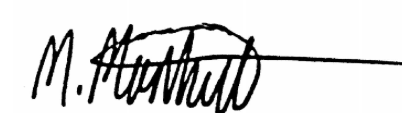
\includegraphics[width=50mm,scale=0.5]{figures/sig.png}\newline

\noindent
Imperial College London\newline

The copyright of this thesis rests with the author and is made available under a Creative Commons Attribution Non-Commercial No Derivatives licence. Researchers are free to copy, distribute or transmit the thesis on the condition that they attribute it, that they do not use it for commercial purposes and that they do not alter, transform or build upon it. For any reuse or redistribution, researchers must make clear to others the licence terms of this work.


\chapter*{Executive summary}

\chapter*{Acknowledgements}

\chapter*{List of Publications and Presentations}

\section*{Publications}

\section*{Oral Presentations}
\begin{enumerate}
    \item \textbf{M. Plunkett}, A. Murugan, K. Li; A hydrogen impurity enrichment device using Pd-Alloy membranes to support the hydrogen economy. Presented at International Conference for Membrane and Electromembrane Processes 2018, 13th – 16th May 2018, Prague, Czech Republic. t
    \item \textbf{M. Plunkett}, A. Murugan, K. Li; A hydrogen impurity enrichment device using Pd-Alloy membranes to support the hydrogen economy. Presented at 15th International Conference on Inorganic Membranes, 18th – 22nd June 2018, Dresden, Germany. 
    \item \textbf{M. Plunkett}; The use of hydrogen selective materials for quality assurance of fuel grade hydrogen to ISO 14687-2 . Presented at 2nd bi-annual Gas and Particle Metrology symposium, 14th August, 2018, Teddington, United Kingdom 
\end{enumerate}

\chapter*{List of Figures}

\chapter*{List of Tables}

\chapter*{List of Acronyms, Abbreviations and Symbols}


\tableofcontents



\chapter{Introduction}
\section{Problem statement}
Due to the damaging environmental effects of using fossil fuels in the transport sector, national and international targets have been set in order to reduce global CO2 emissions. In the UK for example, there is a plan to completely ban the sales of new conventional petroleum vehicles by as early as 2040. 1 One proposed solution is further adoption of fuel cells and other energy generation methods which utilize hydrogen as a carbon free energy source. 

Despite the fact that the technology for hydrogen powered fuel cells, in particular proton exchange membrane fuel cells, has existed since the early 1960’s their application has been limited to providing power for space missions and other niche applications. It wasn’t until the late 90’s where developments in lowering platinum catalyst loading and the production of thin film electrodes drove the cost of fuel cells down to a level where they were a realistic option for transportation. As of 2017, a number of auto mobile manufacturers including Toyota,2 Hyundai, 3 Honda 4 and Daimler 5 now offer hydrogen vehicles commercially and it is becoming increasingly possible to retrofit a petroleum vehicle to run off hydrogen. 6 Many countries in the EU and globally have ambitious hydrogen infrastructure plans over the next 10 years in an effort to become less reliant on importing fossil fuels, increase their energy security, and transition to a carbon free energy system.

The development of the hydrogen economy is still in its infancy in Europe, but several countries are aiming to employ sizable hydrogen fuelling infrastructures over the next few decades. National reports state that Europe’s position in 2030 will be: UK - 1,100 hydrogen refuelling stations and 1.6 million fuel cell vehicles 7, France – 600 hydrogen refuelling stations and 0.8 million fuel cell vehicles 8, Germany – 1,180 hydrogen refuelling stations and 1.8 million fuel cell vehicles 9 and the Netherlands – 200 hydrogen refuelling stations and 0.2 million fuel cell vehicles. 9 The fuel cell system in a hydrogen vehicle can easily degrade if even parts-per-billion to parts-per-million level of some impurities are present in the hydrogen. Therefore, it is imperative that hydrogen purity, and techniques for verifying the purity, are adequate to ensure customers vehicles are not inadvertently damaged by fluctuations in hydrogen composition. 

International standards dictate that it is mandatory for all hydrogen suppliers to prove that their product is pure enough to prevent degradation of fuel cell components. The international standard ISO 14687-2:2012 10 shown in Table 1 specifies the maximum impurity levels of 13 impurities that are permissible in fuel cell hydrogen. ISO 14687-2:2012 include some challenging hydrogen purity specifications mainly due to the low limits of detection of standard techniques used to measure the compounds included in the standard. 

Existing hydrogen purity laboratories are unable to perform traceable analysis to ISO 14687 specifications because appropriate methods and standards have not been developed. The consequence of this is that hydrogen suppliers cannot provide evidence that their fuel meets the International Standard and therefore are not permitted to supply hydrogen. Of the 13 gaseous impurities listed in ISO 14687-2, there is no single method for measuring all impurities. Laboratories must therefore use several instruments to perform such an analysis.  In 2015 Murugan et al published a review of methods for analysing the purity of fuel grade hydrogen 11. They concluded that in order for a single laboratory to provide full hydrogen analysis to ISO 14687-2 specifications it would need to comprise a variety of instruments including GCs, FTIR and CRDS. The capital cost of purchasing the gas analysers to perform analysis on the measurable impurities in a hydrogen sample can amount to >€500,000 11 and hence performing analysis would be out of reach for many of the smaller laboratories. 

While the impurities listed in ISO 14687-2 are specified at extremely low amount fractions, many can be analysed at higher amount fractions through the use of cheap and routine gas analysers such as GC-MS. A potential solution to this would be to increase the concentration above the limit of detection of one of these cheaper analysers. These techniques are referred to as enrichment or pre-concentration. The most commonly used technique for pre-concentration of hydrogen fuel samples is referred to as ‘Hydrogen Impurity Enrichment’.  This method involves passing the sample through a palladium or palladium alloy membrane which is heated to 400OC. Palladium as a membrane material only allows the passage of hydrogen, and as hydrogen leaves the system, the impurities remain, increasing in time as more hydrogen permeates through the membrane.  This increase in concentration is referred to as the enrichment factor and. Once the enrichment is complete the sample can then be analysed at these higher concentrations, and using the enrichment factor, the original composition of the sample can be found. 

In order for these devices to provide accurate results the behaviour of the membrane material, and its interaction with any impurities present in the hydrogen same, must be properly understood.  


\section{Research Background}
\subsection{Hydrogen Production}
Hydrogen production refers to a range of industrial processes for generating hydrogen. Since there are no natural reserves of hydrogen all hydrogen must be obtained through one of these methods. The most important factor for determining the feasibility of a hydrogen production process is the primary source of energy that is used. Currently the options for this are nuclear energy in the form of heat, renewable energy in the form of heat, electricity, or light, or fossil fuels. Currently the primary sources of hydrogen are from steam reforming of methane and other hydrocarbons which in total accounts for 96\% of global hydrogen production, with electrolysis of water accounting for the remaining 4\%.
\subsubsection{Hydrogen from fossil fuels and hydrocarbons}

\subsubsection{Hydrogen from water}

\chapter{Literature review}

\chapter{Density functional theory as a screening method for dense metallic membranes}

\chapter{Impurity resistance of dense metal membranes under hydrogen impurities}

\chapter{A hydrogen impurity measurement device for validating ISO 14687 standard}

\chapter{Conclusion and future work}
\end{document}